\def\qI{\ensuremath{\mathcal{I}}}
\def\TT{\ensuremath{\mathrm{TT}}}
\def\fGW{\ensuremath{f_{\mathrm{GW}}}}

In this chapter we briefly review the theory of gravitational waves: how they arise in \ac{GR} and how they can be detected by an interferometer. We then review the physics behind the \ac{LIGO} and Virgo interferometers, including their main sources of noise. Finally, we examine potential sources of \ac{GW} waves that can be detected by the \ac{LIGO} and Virgo interferometers.

\section{Gravitational Waves in General Relativity}

We begin our discussion with Einstein's field equations, given by\footnote{We will work in ``natural units" in which $G = c = 1$, where $G$ is Newton's gravitational constant and $c$ is the speed of light.}:

\begin{equation}
\label{eqn:einstein_field_eqns}
R_{\alpha \beta} - \frac{1}{2}R g_{\alpha\beta} = 8\pi T^{\alpha \beta}
\end{equation}
Here, $R_{\alpha \beta}$ is the Rici tensor, $R$ is the Rici scalar, $g_{\alpha \beta}$ is the metric tensor, and $T^{\alpha \beta}$ is the stress-energy tensor.


\subsection{Gravitational Waves from a Compact Binary Inspiral}

We now consider the gravitational radiation emitted from a system consisting of two compact objects orbiting around each other. Let the mass of the objects be denoted by $m_1$ and $m_2$, such that the total mass, $M$, is $M = m_1 + m_2$, and consider their motion when they are at a distance $a \gg 2M$. We will assume their motion is determined entirely by their mutual gravitational attraction and that $m_1 ~ m_2 ~ \Msun$. Although we will find that the orbit of the objects shrinks due to the energy loss from emitted \acp{GW}, with these assumptions, $\dot{a} \ll v_{\mathrm{tan}}$. Thus we can use Kepler's laws to evaluate the dynamics of the binary; the orbital angular velocity is therefore:
\begin{equation}
\label{eqn:orbit_ang_v}
\omega = \sqrt{\frac{M}{a^3}}
\end{equation}

% need to show where this equation comes from
From equation \ref{eqn:?} the dominant contribution to the gravitational wave field is given by the mass-quadrupole term:
\begin{equation}
\label{eqn:h_mass_quad}
h^{\TT}_{jk} = \frac{2}{r} \ddot{\qI}^\TT(t - r)
\end{equation}
where $t$ is the time coordinate, $r$ is the radial coordinate, and the quadrupole moment, $\qI$, is given by:
\begin{equation}
\label{eqn:quad_moment}
\qI = \int \rho(\mathbf{x})\left( x_j x_k - \frac{1}{3} \delta_{jk} \delta_{mn} x^{m} x^{n} \right) \d^3 x
\end{equation}

To evaluate the amplitude of the \ac{GW} field we must first evaluate $\qI$. Since we only have two masses, we can use the discreet form of the quadrupole moment to directly write:
\begin{equation}
\label{eqn:discreet_qm}
\qI_{ij} = m_1(x_{1i}x_{1j} - \delta_{ij}\frac{1}{3} r_1^2) + m_2(x_{2i}x_{2j} - \delta_{ij}\frac{1}{3}r_2^2)
\end{equation}
where $r_n^2 = x_n^2 + y_n^2$ is the radial position of the $n\th$ mass. Working in the center-of-mass frame of the binary (see figure \ref{fig:binary_com_diagram}), we have:
\begin{align*}
x_1 &= r_1 \cos \omega t \\
y_1 &= r_1 \sin \omega t \\
x_2 &= - r_2 \cos \omega t \\
y_2 &= - r_2 \sin \omega t \\
\end{align*}
where
\begin{align}
r_1 &= a\frac{m_2}{m_1 + m_2} \\
r_2 &= a \frac{m_1}{m_1 + m_2}
\end{align}
Plugging these values into equation \ref{eqn:discreet_qm} we have:
\begin{align}
\qI_{xx} &= m_1 x_1^2 + m_2 x_2^2 - \frac{1}{3}(m_1r_1^2 + m_2r_2^2) \nonumber \\
         &= (m_1r_1^2 + m_2r_2^2)\left(\cos^2 \omega t - \frac{1}{3}\right) \nonumber \\
         &= a^2\left(\frac{m_1m_2^2 + m_2m_1^2}{m_1+m_2}\right)\left(\cos^2 \omega t - \frac{1}{3}\right) \nonumber \\
         &= \mu a^2 \left(\cos^2 \omega t - \frac{1}{3} \right)
\end{align}
where:
\begin{equation}
\label{eqn:reduced_mass}
\mu = \frac{m_1 m_2}{M}
\end{equation}
is the reduced mass. By a similar calculation, we get:
\begin{align}
\qI_{yy} &= \mu a^2 \left(\sin^2 \omega t - \frac{1}{3}\right) \\
         &= -\qI_{xx} \\
\qI_{zz} &= -\frac{1}{3} \mu a^2 \\
\qI_{xy} &= \mu a^2 \cos \omega t \sin \omega t \\
         &= \qI_{yx}
\end{align}
The second time derivative of the quadrupole moment is thus:
\begin{subequations}
\begin{align}
\ddot{\qI}_{xx} &=  -2\mu a^2\omega^2 \cos(2\omega t) \\
\ddot{\qI}_{yy} &=  2\mu a^2\omega^2 \cos(2\omega t)  \\
\ddot{\qI}_{xy} &=  -2 \mu a^2 \omega^2 \sin(2 \omega t) \\
                &=  \ddot{\qI}_{yx} \\
\ddot{\qI}_{zz} &=  0
\end{align}
\label{eqn:second_deriv_qm}
\end{subequations}

In order to plug equations \ref{eqn:second_deriv_qm} into equation \ref{eqn:h_mass_quad} we need the transverse part of the moments. We know that the gravitational waves will propagate outward from the binary. Therefore, if we project equations \ref{eqn:second_deriv_qm} into the spherical coordinates $\{r,\iota,\phi\}$ shown in figure \ref{fig:?}, then $\qI_{\iota\iota},~\qI_{\phi\phi},$ and $\qI_{\iota\phi}~ (= \qI_{\phi\iota})$ will form parts of the tensor transverse transverse to the propagation. Since the $z$ components of the time derivative of the quadrupole are all zero, the transformation law is simplified to:
\begin{align*}
\ddot{\qI}_{i'j'}  &= \Lambda\indices{_{i'}^i} \Lambda\indices{_{j'}^j} \ddot{\qI}_{ij} \\
            &= \Lambda\indices{_{i'}^x} \Lambda\indices{_{j'}^x} \ddot{\qI}_{xx} + \Lambda\indices{_{i'}^x} \Lambda\indices{_{j'}^y} \ddot{\qI}_{xy} + \Lambda\indices{_{i'}^y} \Lambda\indices{_{j'}^x} \ddot{\qI}_{yx} + \Lambda\indices{_{i'}^y} \Lambda\indices{_{j'}^y} \ddot{\qI}_{yy}
\end{align*}
We can further simplify the problem by setting the initial orbital phase, $\phi$, to 0. Since we have assumed quasi-stationary circular orbits, we can later account for arbitrary initial phase by letting $\omega t \rightarrow \omega t + \phi$. Doing so simplifies the transformation matrix to:
\begin{equation*}
\Lambda = \begin{pmatrix}
    \sin \iota &    0    &  \cos \iota \\
    \cos \iota &    0    &  -\sin \iota \\
         0     &    1    &    0
    \end{pmatrix}
\end{equation*}
Resulting in:
\begin{align*}
\ddot{\qI}_{\iota\iota} &= \ddot{\qI}_{xx} \cos^2\iota \\
\ddot{\qI}_{\phi\phi}   &= \ddot{\qI}_{yy} \\
\ddot{\qI}_{\iota\phi}  &= \ddot{\qI}_{xy} \cos \iota \\
                        &= \ddot{\qI}_{\phi\iota}
\end{align*}
To make the tensor traceless in this coordinate basis, we set $\ddot{\qI}^{\TT}_{\iota\iota} = -\ddot{\qI}^{\TT}_{\phi\phi} = 1/2(\ddot{\qI}_{\iota\iota} - \ddot{\qI}_{\phi\phi})$. Letting $\omega t \rightarrow \omega t - \phi$, we have:
\begin{align}
\ddot{\qI}^{\TT}_{\iota\iota} &= \mu a^2 \omega^2 \cos(2[\omega t - \phi])(1 + \cos^2\iota) \\
\ddot{\qI}^{\TT}_{\iota\phi}  &= -2 \mu a^2 \omega^2 \sin(2[\omega t - \phi])\cos\iota
\end{align}
Plugging this into equation \ref{eqn:h_mass_quad}, and using Kepler's law to put $a$ in terms of $M$ and $\omega$ ($a = \left(M/\omega^2\right)^{1/3}$), we have:
\begin{subequations}
\label{eqn:h_pls-h_crs}
\begin{align}
h^{\TT}_{\iota\iota} &= \frac{2}{r}\mu (M \omega)^{2/3} \cos(2[\omega (t-r) - \phi])(1 + \cos^2\iota) &= h_{\pls} \\
h^{\TT}_{\iota\phi}  &= -\frac{4}{r} \mu (M\omega)^{2/3} \sin(2[\omega (t-r) - \phi])\cos\iota &= h_{\crs}
\end{align}
\end{subequations}
Here we have identified the $\iota\iota$ and $\iota\phi$ parts of the \ac{GW} field as the ``plus" and ``cross" polarizations by using the basis vectors \cite{ref:BlanfordThorne}:
\begin{equation}
\mathbf{e}^{\pls} = (\vec{e}_{\iota} \otimes \vec{e}_{\iota} - \vec{e}_{\phi} \otimes \vec{e}_{\phi}), ~ \mathbf{e}^{\crs} = (\vec{e}_{\iota} \otimes \vec{e}_{\phi} + \vec{e}_{\phi} \otimes \vec{e}_{\iota})
\end{equation}
In equations \ref{eqn:h_pls-h_crs} we can see that the \emph{gravitational-wave frequency} is \emph{twice} the orbital frequency:
\begin{equation}
\label{eqn:f_GW}
\fGW = 2 f_{\mathrm{orbit}} = \frac{\omega}{\pi}
\end{equation}

The inclination angle, $\iota$, and the distance to the center of mass, $r$, are \emph{extrinsic} parameters of the binary: they depends only on the orientation of the binary with respect to an outside observer. To separate the part of the waveform that depends on the \emph{intrinsic} parameters of the binary --- i.e., the physical parameters of the binary that are independent of the location of the observer\footnote{When we say ``independent of the location of the observer" we mean independent of the location of any observers that are in the same \ac{LLF}.} --- we define the \emph{sine chirp}, $h_s$, and the \emph{cosine chirp}, $h_c$ \cite{ref:Brown}:
\begin{subequations}
\label{eqn:cos_sin_chirp}
\begin{align}
h_c &\equiv 2 \mu (M \omega^{2/3}) \cos(2[\omega t - \phi_0] ) \\
h_s &\equiv 2 \mu (M \omega^{2/3}) \sin(2[\omega t - \phi_0] )
\end{align}
\end{subequations}
such that:
\begin{align}
h_\pls &= \frac{h_c}{r} (1 + \cos^2\iota) \\
h_\crs &= \frac{h_s}{r} \cos\iota
\end{align}
(The reason for the name ``chirp" will become clear below.) Here, $\phi_0$ is the phase of the binary at some initial point in time.

\subsection{Evolution of the Gravitational Waveform in Newtonian Physics}

In Chapter \ref{ch:pipeline_principles} we will find that we use the sine and cosine waveforms to \emph{match-filter} data from \ac{GW} detectors. Match filtering offers the best way to find a \ac{CBC} \ac{GW} signal that is buried in noise. However, to perform the match filter, we need to generate a time or frequency series for the waveform. From equations \ref{eqn:cos_sin_chirp} we see that this requires knowledge of how the orbital phase, $\omega t$, (or, via equation \ref{eqn:f_GW}, the gravitational-wave phase) evolves with time (or frequency). We can find this by considering the energy lost by the binary due to gravitational radiation.

The energy loss from \ac{GW} emmision is given by \cite{ref:BlanfordThorne}:
\begin{equation}
\label{eqn:energy_loss-t}
\frac{\d E}{\d t} = -\frac{1}{5}\left< \dddot{\qI}_{jk} \dddot{\qI}^{jk} \right>
\end{equation}
where the brackets $<\cdot>$ denote an average over time. Using equations \ref{eqn:second_deriv_qm}, we find:
\begin{align*}
\dddot{\qI}_{xx} &= 4 \mu a \omega^3\sin(2\omega t) &= -\dddot{\qI}_{yy} \\
\dddot{\qI}_{xy} &= -4 \mu a^2 \omega^3\cos(2\omega t) &= \dddot{\qI}_{yx}
\end{align*}
This gives:
\begin{align*}
\frac{\d E}{\d t} &= -\frac{2}{5}\left< \ddot{\qI}_{xx}^2 + \ddot{\qI}_{xy}^2 \right> \\
    &= -\frac{32}{5} \mu^2 a^4 \omega^6 \left< \sin^2(2\omega t) + \cos^2(2\omega t) \right> \\
    &= -\frac{32}{5} \frac{\mu^2 M^3}{a^5}
\end{align*}
In the last step we have again used Kepler's law to put $\omega$ in terms of $M$ and $a$. We can use this equation to find how the separation distance shrinks with time. Using the chain rule we have:
\begin{equation}
\label{eqn:energy_loss-a}
\frac{\d E}{\d t} = \frac{\partial E}{\partial a}\frac{\d a}{\d t}
\end{equation}
From Newton's law of gravity and conservation of energy, the binary's energy is related to the separation distance by:
\begin{equation*}
\frac{\partial E}{\partial a} = \frac{\mu M}{2a^2}
\end{equation*}
Plugging this into equation \ref{eqn:energy_loss-a} yields:
\begin{equation*}
\frac{1}{2} a^3 \d a = -\frac{32}{5} \mu M^2 \d t
\end{equation*}
Integrating this from some initial separation, $a_0$, at time $t_0$, to the separation, $a$, at some arbitrary time $t$ gives:
\begin{equation}
\label{eqn:a_evolution}
a = a_0 \left(1 - \frac{t-t_0}{\tau_0} \right)^{1/4}
\end{equation}
where:
\begin{equation}
\label{eqn:tau_0-a}
\tau_0 = \frac{5}{256} \frac{a_0^4}{\mu M^2}
\end{equation}
is the \emph{time to coalescence}. That is, $\tau_0$ is the amount of time it takes for the binary to go from the initial separation $a_0$ to $a=0$. In equation \ref{eqn:a_evolution} we can see that the orbital separation decreases with time due to the loss in energy. In other words, the two masses ``inspiral" into each other.

We can use equations \ref{eqn:a_evolution} and \ref{eqn:tau_0-a}, and Kepler's third law to find how the orbital angular velocity changes with time. Re-arranging equation \ref{eqn:keplers_thirdlaw} to $a = (M/\omega^2)^{1/3}$ and manipulating equation \ref{eqn:tau_0-a} to get $a_0$ in terms of $\tau_0$, we have, from equation \ref{eqn:a_evolution}:
\begin{equation*}
M^{4/3}\omega^{-8/3} = \frac{256}{5} \mu M^2(\tau_0 - t)
\end{equation*}
Here, we have set the initial time $t_0 = 0$. Rearranging, we have:
\begin{equation}
\label{eqn:omega_evolution}
\omega = \left[ \frac{5}{256} \frac{1}{\eta M^{5/3}(\tau_0 - t)} \right]^{3/8}
\end{equation}
where:
\begin{equation}
\label{eqn:symmetric_mass}
\eta \equiv \frac{\mu}{M}
\end{equation}
is the \emph{symmetric mass-ratio}. Using equation \ref{eqn:f_GW} to relate the gravitational-wave frequency to $\omega$, we find:
\begin{equation}
\label{eqn:f_evolution}
\fGW(t) \propto (\tau_0 - t)^{-3/8}
\end{equation}
Figure \ref{fig:GW_evolution-freq} shows what the gravitational wave-frequency looks like as a function of time. We see that the wave sweeps upward in frequency in a ``chirp" pattern, asymptoting to infinity as $a \rightarrow 0$.

We can also use equation \ref{eqn:omega_evolution} to find how the amplitude of the waveform changes over time. In equations \ref{eqn:cos_sin_chirp} we see that the amplitude of the waveform is proportional to $M\omega^{2/3}$. Thus:
\begin{equation}
\label{eqn:amp_evolution}
|h_c| = |h_s| = 2 \left( \frac{5}{256} \frac{\mchirp}{\tau_0 - t} \right)^{1/4}
\end{equation}
where we have defined the \emph{chirp mass}, $\mchirp$, as:
\begin{equation}
\mchirp \equiv \eta^{3/5}M
\end{equation}
Thus the amplitude also increases with time, asymptoting to infinity as $a \rightarrow 0$. Figure \ref{fig:GW_evolution-waveform} shows what the waveform evolution looks like for $M=1\,\Msun$ and $\eta = 1/4$ (i.e., for an equal-mass binary).

%Note that from the definition in equation \ref{eqn:quad_moment}, the quadrupole and its time derivatives are traceless. 

\subsection{Orbital Dynamics in a Schwarzschild Spacetime}

In the above analysis we assumed the relative velocities of the binary's component masses were small compared to the speed of light, and that the spacetime curvature was relatively flat. This allowed us to use Newtonian and Keplerian dynamics to analyze the binary. While this worked well when the masses were far apart from each other, it breaks down as the separation distance gets small. This was evident in the fact that the orbital angular velocity asymptoted to infinity as $a \rightarrow 0$. This means that the component masses' relative tangential velocity:
\begin{equation}
v = (M\omega)^{1/3}
\end{equation}
would also approach infinity. Clearly there is a separation distance for which our assumptions fail, and we must take into account relativistic effects.

To illustrate relativistic effects, we consider a test-particle with mass $m$ orbiting a massive black hole with mass $M$, such that $m \ll M$. For simplicity we will assume that both the test mass and the black hole have negligible spin. Thus, we can describe the spacetime using the Schwarzchild metric \cite{ref:MTW}:
\begin{equation}
\d s^2 = - (1 - 2M/r)\d t^2 + \frac{\d r^2}{1 - 2M/r} + r^2\d\Omega^2
\end{equation}
where $\d \Omega$ is the solid angle. The coordinates are chosen such that $r=0$ is at the ``center" of the black hole. Without loss in generality we will assume the inclination angle is equal to $\pi/2$, so that the solid angle element reduces to $\d\Omega = r^2\d\phi$.\footnote{For a treatment of this problem with $\iota \neq \pi/2$ see Box 25.4 of \cite{ref:MTW}.} In this case the metric only has three elements:
\begin{subequations}
\begin{align}
g_{tt} &= - (1 - 2M/r) \\
g_{rr} &= (1-2M/r)^{-1} \\
g_{\phi\phi} &= r^2
\end{align}
\end{subequations}

In the last section the equation of motion for the masses was given by Kepler's third law, which related the orbital angular velocity to the mass and separation distance. To analyze the test particle's orbital evolution we again need an equation of motion. However, since we are working in a curved spacetime it is not clear that Kepler's third law still holds. To find the relativistic equation of motion, we consider the particle's geodesic path as it orbits the black hole. Since no external forces act on the particle, the geodesic equation is \cite{ref:MTW, ref:Schutz, ref:Carroll}:
\begin{equation}
\frac{\d^2 x^{\alpha}}{\d \tau^2} + \Gamma\indices{^\alpha_{\mu \nu}} \frac{\d x^{\mu}}{\d\tau} \frac{\d x^{\nu}}{\d\tau} = 0
\end{equation}
where the Christoffel symbol is:
\begin{align}
\label{eqn:christoffel_symbols}
\Gamma\indices{^\alpha_{\mu\nu}} &= g^{\alpha\sigma}\Gamma\indices{_{\sigma\mu\nu}} \nonumber \\
    &= \frac{1}{2}g^{\alpha\sigma}( g_{\sigma\mu,\nu} + g_{\sigma\nu,\mu} - g_{\mu\nu,\sigma}) \nonumber \\
    &= \frac{1}{2}g^{\alpha\alpha}(g_{\alpha\mu,\nu} + g_{\alpha\nu,\mu} - g_{\mu\nu,\alpha})
\end{align}
The ``," indicates the partial derivative of the tensor with respect to the trailing indices. In the last step we have used the fact that there are no mixing terms in the metric (i.e., $g^{\alpha\sigma} = \delta\indices{^{\alpha}_\sigma}g^{\alpha\sigma}$). 

Before analyzing these equations, we note a few properties of the metric which greatly simplify the problem. The metric has no $t$, $\phi$, or (since we set the particle's inclination angle to $\pi/2$) $\iota$ dependence. Thus the $t$, $\phi$, and $\iota$ components of the particle's conjugate four-momentum, $p_\alpha$ are conserved \cite{ref:MTW, ref:Schutz, ref:Carroll}. The particle's four-momentum is given by:
\begin{equation}
p^{\alpha} = m u^{\alpha} = m \frac{\d x^\alpha}{\d\tau}
\end{equation}
where $u^{\alpha}$ is the particle's four-velocity. The four-momentum is related to the conjugate momentum by: $p^{\alpha} = g^{\alpha\beta}p_{\alpha}$. Since $p_{\alpha}$ has no $\tau$ dependence, and since $g^{\alpha\beta}$ only depends on $r$, $\dot{p}^{\alpha} \sim \dot{r}$. (Dots over the coordinates indicate differentation with respect to the proper time.) We shall assume, as we did in the previous section, that $\dot{r} \ll \dot{\phi}$, i.e., that the particle follows quasi-stationary orbits. In this case, $\dot{r} \approx 0$, as well as $\ddot{r}$. Thus: 
\begin{equation}
\dot{p}^t = \ddot{t}/m = \dot{p}^\phi = \ddot{\phi}/m = \dot{p}^\iota = \ddot{\iota}/m = 0
\end{equation}
Since we have fixed the inclination angle to $\pi/2$, $\ddot{\iota}$ is also zero. From equation \ref{eqn:christoffel_symbols}, this means that $\Gamma^{\iota}_\mu\nu$ is zero, and so the $\iota$ equation of motion gives the trival result $0 = 0$. Thus we only have three equations to consider:
\begin{equation}
\label{eqn:equations_of_motion}
\Gamma\indices{^\alpha_{tt}} \dot{t}^2 + 2\Gamma\indices{^\alpha_{t\phi}}\dot{t}\dot{\phi} + \Gamma\indices{^\alpha_{\phi\phi}} \dot{\phi}^2 = 0 
\end{equation}
where $\alpha = r,t,\phi$. We further simplify these equations by noting:
\begin{align*}
\Gamma\indices{^\alpha_{tt}} &= \frac{1}{2} g^{\alpha\alpha}(2g_{\alpha t,t} - g_{tt,\alpha}) &= -\frac{1}{2} g^{\alpha\alpha}g_{tt,\alpha} \\
\Gamma\indices{^\alpha_{\phi\phi}} &= \frac{1}{2} g^{\alpha\alpha}(2g_{\alpha \phi,\phi} - g_{\phi\phi,\alpha}) &= -\frac{1}{2} g^{\alpha\alpha}g_{\phi\phi,\alpha} \\
\Gamma\indices{^\alpha_{t\phi}} &= \frac{1}{2} g^{\alpha\alpha}(g_{\alpha t,\phi} + g_{\alpha \phi,t} - g_{t\phi,\alpha}) &= 0 \\
\end{align*}
Since $g_{tt,\alpha}$ and $g_{\phi\phi,\alpha}$ are only non-zero if $\alpha = r$, the only non-zero Christoffel symbols are $\Gamma\indices{^r_{tt}}$ and $\Gamma\indices{^r_{\phi\phi}}$. This means the only non-trival equation of motion is the one for which $\alpha = r$. The non-zero Christoffel symbols are:
\begin{subequations}
\begin{align}
\Gamma\indices{^r_{tt}} &= -\frac{1}{2} g^{rr}g_{tt,r} &= \frac{M}{r^2}(1 - 2M/r) \\
\Gamma\indices{^r_{\phi\phi}} &= -\frac{1}{2} g^{rr}g_{\phi\phi,r} &= -r(1-2M/r)
\end{align}
\end{subequations}
Plugging these into the equation of motion yields:
\begin{align*}
\frac{M}{r^2}(1 - 2M/r)\dot{t}^2 - r(1-2M/r)\dot{\phi}^2 = 0 \\
\Rightarrow \frac{\dot{\phi}^2}{\dot{t}^2} = \frac{M}{r^3}
\end{align*}
Note that:
\begin{equation}
\frac{\dot{\phi}}{\dot{t}} = \frac{\d\phi/\d\tau}{\d t/\d\tau} = \frac{\d\phi}{\d t} = \omega
\end{equation}
where $\omega$ is the angular velocity of the test particle as measured by an observer in the particle's \ac{LLF}. Thus we have:
\begin{equation}
\omega = \sqrt{\frac{M}{r^3}}
\end{equation}
Evidently Kepler's third law is valid for all $r$; i.e., it is a relativistic equation. 

As noted above, $\dot{\phi} = p^\phi/m$ and $\dot{t} = p^t/m$. We can therefore write:
\begin{equation}
\label{eqn:eom1}
\frac{p^\phi}{p^t} = \sqrt{\frac{M}{r^3}}
\end{equation}
Now, since $p_t$ and $p_\phi$ are conserved, we can set them equal to the constants $-E$ and $L$, respectively. We can identify these constants as the particle's energy and momentum as seen by an observer at $r = \infty$ \cite{ref:Schutz}. Raising the indices, we have:
\begin{align}
p^t &= g^{tt}p_t &= \frac{E}{1-2M/r} \\
p^\phi &= g^{\phi\phi}p_\phi &= \frac{L}{r^2}
\end{align}
The equation of motion \ref{eqn:eom} is therefore:
\begin{equation}
\label{eqn:eom2}
\frac{(1-2M/r)L}{r^2E} = \sqrt{\frac{M}{r^3}}
\end{equation}
We can put $L$ in terms of $E$ by noting:
\begin{equation*}
p^{\alpha}p^{\beta}g_{\alpha\beta} = p^{\alpha}p_{\alpha} = m^2 u^{\alpha}u_{\alpha} = -m^2
\end{equation*}
Since $p^r$ and $p^\iota$ are both zero,
\begin{equation*}
p^{\alpha}p_{\alpha} = p^t p_t + p^\phi p_\phi = -\frac{E^2}{1-2M/r} + \frac{L^2}{r^2} = -m^2
\end{equation*}
Rearranging this gives:
\begin{equation}
L = r\sqrt{\frac{E^2}{1-2M/r} - m^2}
\end{equation}
Plugging this into equation \ref{eqn:eom2} yields:
\begin{equation}
\label{eqn:Eschwarz}
E = m\frac{1-2M/r}{\sqrt{1-3M/r}}
\end{equation}
We have arrived at a solution for the particle's energy as a function of its oribital distance. (Note that as $r\rightarrow \infty$, $E \rightarrow m$, meaning $E$ becomes the rest-mass energy of the particle, as expected.) 

Figure \ref{fig:Eofr} shows a plot of $E/m$ as a function of $r/M$. From this (or by taking the derivative of equation \ref{eqn:Eschwarz} and setting it equal to zero) we can see that $E/m$ decreases monontonically from inifinity, until it reaches a minimum at $r=6M$. Keep in mind that we obtained this graph by considering quasi-stationary circular orbits. Thus the plot shows how much energy is needed at each $r$ for the particle to maintain a circular orbit. This means that at radii $\geq 6M$ the particle can sustain stable circular orbits without needing any additional energy. Below $r=6M$, however, energy must be added to the particle in order for it to sustain its orbit.\footnote{And below $r=2M$ an infinite amount of energy would be needed for the particle to sustain a stable orbit. Thus $r=2M$ is the event horizon of the black hole, also known as the Schwarschild radius.} Assuming the system evolves adiabatically (that is, no external energy is added), after the particle passes $r=6M$ it will cease to inspiral and will plunge into the black hole. This part of the evolution is known as ``merger."

The point $r=6M$ is known as \ac{ISCO}. At this point our analysis, both in this section and the last, breaks down since we can no longer assume $\dot{r} \ll \dot{\phi}$. The phase and amplitude evolution of the gravitational wave emitted after this point must therefore be evaluated using more sophisticated techniques. Although we found this radius by considering a Schwarschild metric, an \ac{ISCO} will exist for equal-mass systems as well (it may not occur at $r=6M$, however).

The systems we will consider in this thesis have masses low enough that the frequencies of their emitted \acp{GW} are of order a few kHz when they pass \ac{ISCO}. Since our gravitational-wave detectors have low sensitivity at these frequencies (see section \ref{sec:interferometers}) we can simply terminate the matched filter at $f_{\mathrm{isco}}$, which is the frequency of the gravitational wave when the source's component masses pass \ac{ISCO}. This permits us to use the techniques outlined in the last section and the next to generate a \ac{GW} waveform.

\begin{figure}[tbp]
\center
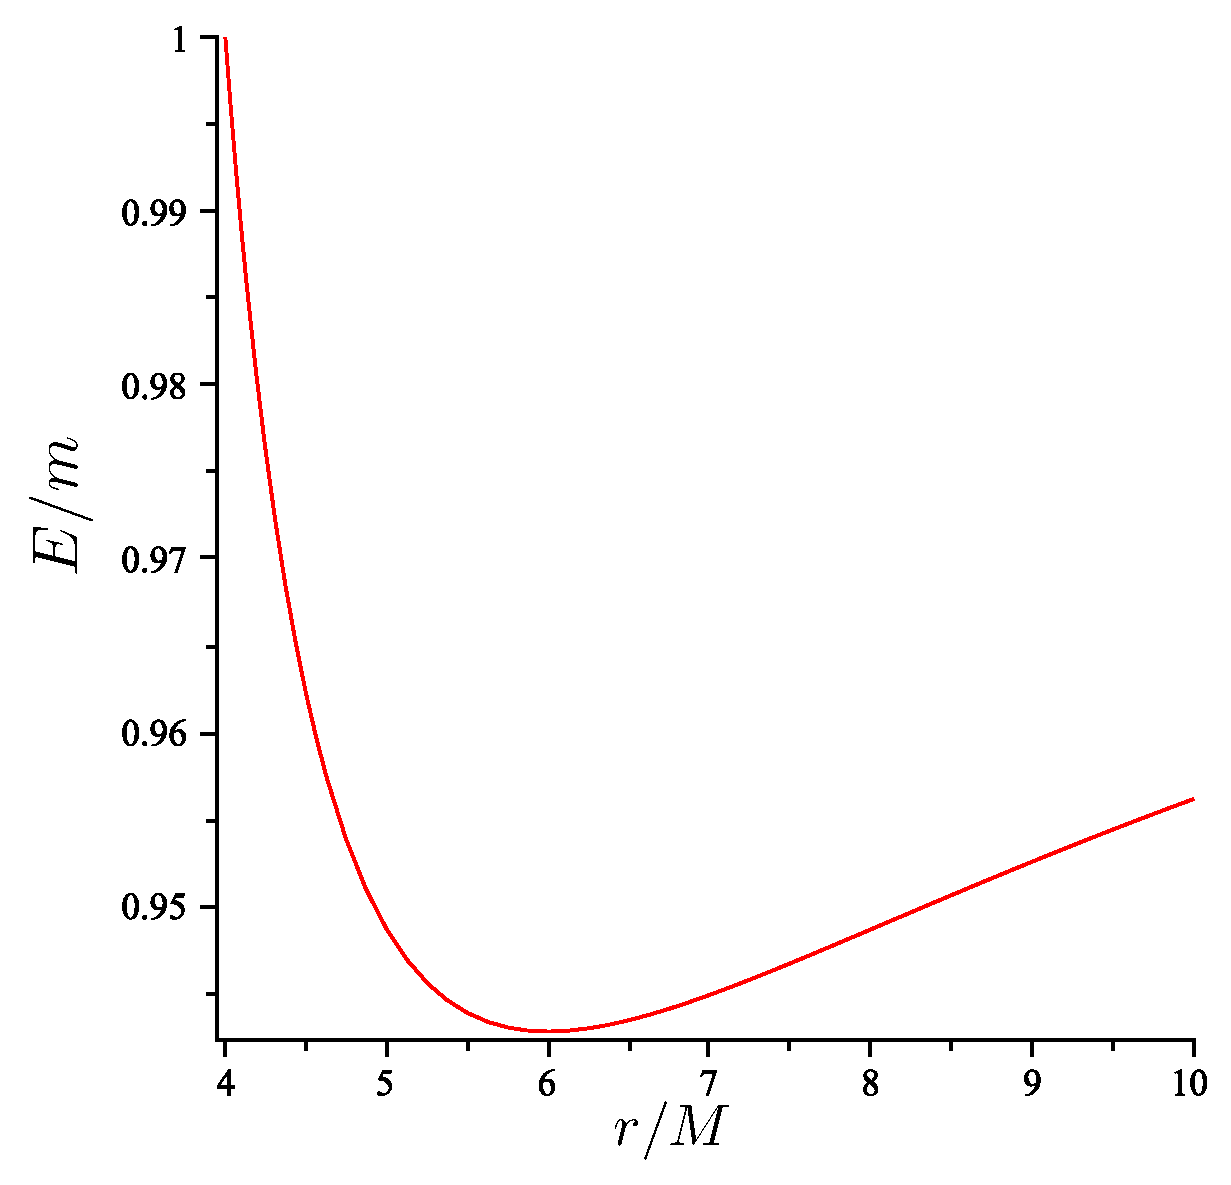
\includegraphics[width=4in]{figures/Eofrplot.pdf}
\caption{A plot of the energy-per-unit mass of a test particle orbiting a Schwarschild black hole as a function of its radial coordinate per the black hole's mass. The plot was created in Maple using equation \ref{eqn:Eschwarz}.}
\end{figure}

\subsection{The Post-Newtonian Expansion}


